\documentclass[aspectratio=169,11pt]{beamer}
\usepackage[T1]{fontenc}
\usepackage[utf8]{inputenc}
\usepackage{lmodern,amsmath,amssymb,graphicx}
\DeclareUnicodeCharacter{2013}{\ensuremath{-}}
\usetheme{default}
\usefonttheme{serif}
\setbeamercolor{normal text}{fg=black,bg=white}
\setbeamercolor{structure}{fg=black}
\setbeamercolor{frametitle}{fg=black}
\setbeamercolor{title}{fg=black}
\setbeamertemplate{navigation symbols}{}
\setbeamertemplate{footline}[frame number]
\setbeamertemplate{itemize items}[circle]
\setbeamersize{text margin left=8mm,text margin right=8mm}
\setlength{\parskip}{5pt}
\newcommand{\db}{\bar\partial}
\newcommand{\C}{\mathbb C}
\newcommand{\R}{\mathbb R}
\newcommand{\Z}{\mathbb Z}
\newcommand{\A}{\mathcal A}
\newcommand{\F}{\mathcal F}
\newcommand{\Lie}{\mathcal L}
\newcommand{\ee}{e_{n,m}}
\newcommand{\Dbar}{D_{\bar z}}
\newcommand{\src}[1]{\par\vfill{\scriptsize #1\par}}
\title{Lecture 12}
\subtitle{The \texorpdfstring{$\bar\partial$}{dbar}-Poincar\'e lemma in one variable}
\author{Daniel Gonz\'alez Casanova Azuela}
\date{}
\hypersetup{pdfauthor={Daniel Gonzalez Casanova Azuela},
 pdftitle={Lecture 12: The dbar-Poincare lemma in one variable}}

\begin{document}
\begin{frame}
\titlepage
\end{frame}

\section{Reminder and plan}
\begin{frame}{Reminder: Dolbeault's theorem}
\[
 H^q(M,\Omega^p_M)\cong H^{p,q}_{\db}(M).
\]
Use the resolution
\[
 0\longrightarrow\Omega^p_M\longrightarrow\A^{p,0}_M
 \xrightarrow{\db}\A^{p,1}_M\xrightarrow{\db}\cdots.
\]
\begin{itemize}
\item \textbf{Exactness:} the $\db$-Poincar\'e lemma gives local primitives.
\item \textbf{Acyclicity:} the sheaves of smooth forms are fine
(Voisin, Definition 4.35 and Proposition 4.36).
\item \textbf{Voisin, Proposition 4.32:} an acyclic resolution computes
sheaf cohomology from its global sections.
\end{itemize}
The missing input is the $\db$-Poincar\'e lemma.
\src{Voisin, \emph{Hodge Theory and Complex Algebraic Geometry I}, Chapter 4.}
\end{frame}

\begin{frame}{Today's theorem: one complex variable}
\textbf{The $\db$-Poincar\'e lemma (local form).}
If $\eta$ is a smooth $(0,1)$-form near a point of $\C$, then
on a smaller disk there is a smooth function $u$ such that
\[
 \db u=\eta.
\]
More precisely, if $\eta$ is smooth on a neighbourhood of a closed disk
$\overline D$, we will construct $u$ on $D$.

For $z=x+iy$,
\[
 \eta=g\,d\bar z,\qquad
 \db u=\frac12(u_x+i u_y)\,d\bar z.
\]
Every $(0,1)$-form is $\db$-closed.
The $(1,1)$ case follows from the same scalar equation.
\end{frame}

\begin{frame}{Next lecture}
\textbf{Several-variable $\db$-Poincar\'e lemma.}
For a smooth $(p,q)$-form $\eta$ on a complex manifold,
\[
 q>0,\quad\db\eta=0
 \quad\Longrightarrow\quad
 \eta=\db\beta\ \text{locally},
 \qquad \beta\text{ of type }(p,q-1).
\]
This completes the local exactness needed for Dolbeault's theorem.

\textbf{Hartogs extension.}
Let $n\geq2$ and $K\subset\C^n$ be compact with $\C^n\setminus K$
connected. Every holomorphic function on $\C^n\setminus K$
extends uniquely to a holomorphic function on $\C^n$.
\src{Verbitsky, Lecture 13: Poincar\'e--Dolbeault--Grothendieck lemma and Hartogs' theorem.}
\end{frame}

\begin{frame}{Huybrechts: the boundary assumption}
All three statements solve $\db\beta=\alpha$ \textbf{throughout $B$}
for $\db$-closed forms of positive antiholomorphic degree.

\medskip
\renewcommand{\arraystretch}{1.45}
\begin{tabular}{@{}p{2.5cm}p{9.8cm}@{}}
\textbf{Statement}&\textbf{Where is the given form smooth?}\\\hline
Prop. 1.3.7&Near the closed disk $\overline B\subset\C$.\\
Prop. 1.3.8&Near the closed polydisk $\overline B\subset\C^n$.\\
Corollary 1.3.9&Only on $B$; no extension across the boundary assumed.
\end{tabular}
\medskip

Here the ``open disk'' in Corollary 1.3.9 is a \textbf{polydisk}:
a product of disks in $\C^n$.

One variable $\longrightarrow$ several variables
$\longrightarrow$ remove the boundary-extension assumption.

A smooth form on $B$ can be unbounded near its boundary.
\src{Huybrechts, \emph{Complex Geometry: An Introduction},\newline
Propositions 1.3.7--1.3.8 and Corollary 1.3.9.}
\end{frame}

\section{Hilbert spaces and Fourier modes}
\begin{frame}{Hilbert spaces: what we need}
A complex \textbf{Hilbert space} is a vector space with an inner product,
complete for the norm $\|v\|=\sqrt{\langle v,v\rangle}$.
We take the inner product linear in its first argument.

Our example is $L^2(0,2\pi]$: square-integrable complex functions,
identified when equal almost everywhere, with
\[
 \langle f,g\rangle=\int_0^{2\pi}f(t)\overline{g(t)}\,dt,
 \qquad \|f\|_2^2=\int_0^{2\pi}|f(t)|^2\,dt.
\]
An \textbf{orthonormal system} $(e_j)$ satisfies
$\langle e_j,e_k\rangle=\delta_{jk}$.
It is an \textbf{orthonormal basis} if its finite linear combinations
are dense in the Hilbert space.

Here ``basis'' allows convergent infinite sums.
\end{frame}

\begin{frame}{Parseval theorem}
Let $H$ be a Hilbert space and $S\subset H$ orthonormal. The following
are equivalent:
\begin{enumerate}
\item $S$ is maximal orthonormal;
\item $\overline{\operatorname{span}(S)}=H$;
\item for every $x\in H$,
\[
 x=\sum_{s\in S}\langle x,s\rangle s;
\]
\item for every $x\in H$,
\[
 \|x\|^2=\sum_{s\in S}|\langle x,s\rangle|^2.
\]
\end{enumerate}
Thus an orthonormal set is a Hilbert basis exactly when its finite
linear combinations are dense.
\end{frame}

\begin{frame}{Parseval: why the series converges}
For $x\in H$, consider
\[
 \sum_{s\in S}\langle x,s\rangle s.
\]
For a finite $S_1\subset S$, Pythagoras gives
\[
 \left\|\sum_{s\in S_1}\langle x,s\rangle s\right\|^2
 =\sum_{s\in S_1}|\langle x,s\rangle|^2.
\]
By Bessel's inequality,
\[
 \sum_{s\in S}|\langle x,s\rangle|^2\leq\|x\|^2.
\]
Hence the numerical sum converges, so the Cauchy criterion shows that
the vector series converges in $H$.
\end{frame}

\begin{frame}{Parseval: maximality means generation}
Let
\[
 y=x-\sum_{s\in S}\langle x,s\rangle s.
\]
Then $y\perp S$. If $S$ is maximal orthonormal, this forces $y=0$;
otherwise $y/\|y\|$ could be added to $S$. Hence
\[
 x=\sum_{s\in S}\langle x,s\rangle s.
\]
Its partial sums lie in $\operatorname{span}(S)$, so
\[
 x\in\overline{\operatorname{span}(S)}.
\]
Conversely, if $S$ is not maximal, there is a unit vector
$y_0\perp S$, hence $y_0\perp\overline{\operatorname{span}(S)}$,
so the closed span cannot be all of $H$.\hfill$\square$
\end{frame}

% Verbatim excerpts of functional-analysis/functional-analysis.tex,
% blob 7fbf692c4d59594856090ef4e0bbea68eeb27022, lines 1031--1045.
% No wording or formulas in the excerpts have been corrected.
\begin{frame}{The Fourier example}
\textbf{Example (verbatim).}
In $L_2(–\pi,\pi)$, the collection (or any subset thereof)
			\[x_n=\frac{1}{\sqrt{2\pi}}e^{int},\qquad n=0,\pm1,\ldots\]
			is an orthonormal set of vectors.
\textbf{Proof.}
For any $n\in\Z$,
				\[\int_{-\pi}^\pi x_n\overline{x}_ndt=\frac{1}{2\pi}\int_{-\pi}^\pi e^{int}\overline{e^{int}}dt=\frac{1}{2\pi}\int_{-\pi}^\pi \Vert e^{int}\Vert^2dt=1,\]
\src{\texttt{functional-analysis/functional-analysis.tex}, ``Orthogonal projections''.}
\end{frame}

\begin{frame}{The Fourier example: proof continued}
\textbf{Proof (continued, verbatim).}
\begingroup\small
and if $m$ is another integer,
				\[\int_{-\pi}^\pi x_n\overline{x}_mdt=\frac{1}{2\pi}\int_{-\pi}^\pi e^{int}\overline{e^{imt}}dt=\frac{1}{2\pi}\int_{-\pi}^\pi e^{(n-m)it}dt=\frac{1}{2\pi}\left[\frac{e^{(n-m)it}}{(n-m)i}\right]_{-\pi}^\pi=0.\]
\endgroup
\medskip
In this last calculation, ``another integer'' means $m\ne n$.

This proves orthonormality. To obtain a basis, we must also prove density.
\src{\texttt{functional-analysis/functional-analysis.tex}, ``Orthogonal projections''.}
\end{frame}

\begin{frame}{The real-valued version}
\textbf{Example (verbatim).}
If we restric out attention to only real-valued functions that are square-integrable on the interval $[-\pi,\pi]$, then the collection (or any subset thereof)
			\begin{align*}
				\frac{1}{\sqrt{2\pi}},&\frac{1}{\sqrt{\pi}}\cos t,\frac{1}{\sqrt{\pi}}\cos 2t,\ldots\\
				&\frac{1}{\sqrt{\pi}}\sin t,\frac{1}{\sqrt{\pi}}\sin 2t,\ldots
			\end{align*}
			is an orthonormal set.
\medskip
We use the complex exponential version in the rest of the lecture.
\src{\texttt{functional-analysis/functional-analysis.tex}, ``Orthogonal projections''.}
\end{frame}

\begin{frame}{From an orthonormal system to a basis}
The same integral over $(0,2\pi]$ shows that
\[
 \phi_n(t)=\frac{e^{int}}{\sqrt{2\pi}},\qquad n\in\Z,
\]
is orthonormal in $L^2(0,2\pi]$.

Let
\[
 A=\operatorname{span}\{e^{int}:n\in\Z\}\subset C(S^1,\C).
\]
To prove that $(\phi_n)$ is a Hilbert basis, it remains to prove
\[
 \overline A^{\,L^2}=L^2(S^1).
\]

This does \emph{not} follow from orthonormality. We use
Stone--Weierstrass.
\src{Verbitsky, Lecture 12, pp. 2--4.}
\end{frame}

\begin{frame}{Completeness: Stone--Weierstrass}
\begin{columns}[T]
\begin{column}{0.72\textwidth}
The Fourier polynomials $A$ satisfy the hypotheses:
\begin{itemize}
\item $A$ is an algebra, since $e^{int}e^{imt}=e^{i(n+m)t}$;
\item $1=e^{i0t}\in A$;
\item $A$ is closed under conjugation, since
      $\overline{e^{int}}=e^{-int}$;
\item $A$ separates points of $S^1$: the function $e^{it}$ already does.
\end{itemize}
Therefore Stone--Weierstrass gives
\[
 \overline A^{\,\|\cdot\|_\infty}=C(S^1,\C).
\]
\end{column}
\begin{column}{0.25\textwidth}
\centering
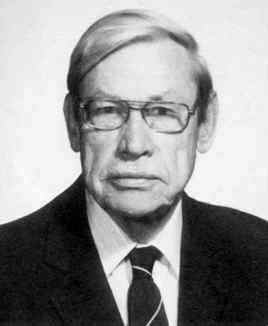
\includegraphics[width=\linewidth]{Stone.jpeg}

\scriptsize Marshall H. Stone
\end{column}
\end{columns}
\end{frame}

\begin{frame}{From uniform density to $L^2$ density}
On $(0,2\pi]$,
\[
 \|f-g\|_2^2
 =\int_0^{2\pi}|f-g|^2dt
 \leq 2\pi\|f-g\|_\infty^2,
\]
hence
\[
 \|f-g\|_2\leq\sqrt{2\pi}\|f-g\|_\infty.
\]
So uniform approximation implies $L^2$ approximation. Therefore
\[
 C(S^1,\C)\subset\overline A^{\,L^2}.
\]

Finally, continuous functions are dense in $L^2(S^1)$, hence
\[
 L^2(S^1)=\overline{C(S^1,\C)}^{\,L^2}
 \subset\overline A^{\,L^2}.
\]
Thus
\[
 \boxed{\overline A^{\,L^2}=L^2(S^1),}
\]
so $(\phi_n)_{n\in\Z}$ is an orthonormal Hilbert basis.\hfill$\square$
\end{frame}

\begin{frame}{The Fourier expansion on the circle}
By the Hilbert-space expansion theorem,
\[
 f(t)=\sum_{n\in\Z}a_n e^{int},\qquad
 a_n=\frac1{2\pi}\int_0^{2\pi}f(t)e^{-int}\,dt.
\]
The sum converges in $L^2$.

From now on we use the normalized measure $dt/(2\pi)$.
Then $e^{int}$ itself has norm one, and the coefficients are simply
its inner products with $f$.

An $L^2$ function on the interval defines a function on the circle
up to a set of measure zero. Smooth functions on the circle correspond
to smooth periodic functions on $\R$.
\end{frame}

\begin{frame}{The Fourier basis on the torus}
Let
\[
 E=\C/(2\pi\Z+2\pi i\Z),\qquad z=x+iy.
\]
Functions on $E$ are periodic in both $x$ and $y$.
For the measure $dx\,dy/(2\pi)^2$, put
\[
 \ee(x,y)=e^{inx+imy},\qquad(n,m)\in\Z^2.
\]
\textbf{Proof that this is a basis.} Orthogonality follows by multiplying
the two one-variable integrals:
\[
 \langle e_{n,m},e_{r,s}\rangle=\delta_{nr}\delta_{ms}.
\]
Their span is again a conjugation-closed algebra containing constants
and separating points of $E$. Stone--Weierstrass and the density of
$C(E)$ in $L^2(E)$ prove completeness.\hfill$\square$
\end{frame}

\begin{frame}{Fourier modes of functions and forms}
Every $f\in L^2(E)$ has the expansion
\[
 f=\sum_{n,m\in\Z}a_{n,m}\ee,\qquad
 a_{n,m}=\frac1{(2\pi)^2}\int_E f(x,y)e^{-inx-imy}\,dx\,dy.
\]
The term $a_{n,m}\ee$ is its $(n,m)$-\textbf{Fourier mode}.
There are two integer indices because there are two real coordinates.

Expand the coefficients of a differential form in the same way:
\[
 \eta=g\,d\bar z=\sum_{n,m}a_{n,m}\ee\,d\bar z.
\]
More generally, a mode is $\ee\alpha$ with $\alpha$ a constant form.
The \textbf{zero mode} is $(n,m)=(0,0)$: its coefficients are constant.
The frequency $(n,m)$ and the form type $(p,q)$ are different indices.
\end{frame}

\section{Differentiation preserves modes}
\begin{frame}{The exterior derivative preserves modes}
\textbf{Claim.} Differentiating a mode keeps the same frequency.

\textbf{Proof.} Direct differentiation gives
\[
 d\ee=\ee(in\,dx+im\,dy).
\]
If $\alpha$ is a constant form, then $d\alpha=0$, so
\[
 d(\ee\alpha)=\ee(in\,dx+im\,dy)\wedge\alpha.
\]
Every coefficient is a multiple of the same basis function $\ee$.\hfill$\square$

The form degree changes; the pair $(n,m)$ does not.
\end{frame}

\begin{frame}{The Dolbeault operator preserves modes}
Our conventions are
\[
 z=x+iy,\qquad I\partial_x=\partial_y,\qquad
 \Dbar=\frac12(\partial_x+i\partial_y),\qquad
 \db=d\bar z\wedge\Dbar.
\]
\textbf{Proof.} Since $\partial_x\ee=in\ee$ and
$\partial_y\ee=im\ee$,
\[
 \db(\ee\alpha)=\frac{in-m}{2}\ee\,d\bar z\wedge\alpha
 \qquad(\alpha\text{ constant}).
\]
Thus $\db$ also preserves each frequency.\hfill$\square$

By uniqueness of Fourier coefficients, if $\db\eta=0$,
each mode of $\eta$ is $\db$-closed. We can seek primitives mode by mode.
For smooth forms, termwise differentiation is justified below.
\end{frame}

\section{Cartan's formula and cohomology}
\begin{frame}{Complex Cartan's formula}
Let $X=\partial_x$ and $IX=\partial_y$ be translation fields on $E$.
Contraction is denoted by $\iota_X$; on a one-form,
$\iota_X\eta=\eta(X)$. Lie derivatives differentiate coefficients.

The real Cartan formula is $d\iota_X+\iota_Xd=\Lie_X$.
Its complex versions are
\[
 \db\iota_X+\iota_X\db
 =\frac12(\Lie_X+i\Lie_{IX}),
\]
\[
 \partial\iota_X+\iota_X\partial
 =\frac12(\Lie_X-i\Lie_{IX}).
\]
With $z=x+iy$ and $IX=\partial_y$, the plus sign belongs to $\db$.
\src{Compare Verbitsky, Lecture 12, p. 13; signs here follow the displayed coordinate conventions.}
\end{frame}

\begin{frame}{Proof of complex Cartan for translations}
For every form $\omega$, the contraction rule gives
\[
 \iota_X(d\bar z\wedge\omega)
 =\underbrace{d\bar z(X)}_{1}\omega-d\bar z\wedge\iota_X\omega.
\]
Also $\Dbar$ commutes with $\iota_X$, since $X$ is constant. Therefore
\begin{align*}
 (\db\iota_X+\iota_X\db)\omega
 &=d\bar z\wedge\iota_X\Dbar\omega
   +\iota_X(d\bar z\wedge\Dbar\omega)\\
 &=\Dbar\omega
 =\tfrac12(\Lie_X+i\Lie_{IX})\omega.
\end{align*}
Replacing $d\bar z,\Dbar$ by $dz,\tfrac12(\partial_x-i\partial_y)$
proves the formula for $\partial$.
Adding the two identities recovers real Cartan.\hfill$\square$
\end{frame}

\begin{frame}{A mode is an eigenvector}
Let $\eta_{n,m}=\ee\alpha$, with $\alpha$ constant.
Since translations leave $\alpha$ fixed,
\[
 \Lie_X\eta_{n,m}=in\eta_{n,m},\qquad
 \Lie_{IX}\eta_{n,m}=im\eta_{n,m}.
\]
For the combination with a minus sign,
\[
 (\Lie_X-i\Lie_{IX})\eta_{n,m}=(in+m)\eta_{n,m}.
\]
The combination used for $\db$ is
\[
 (\Lie_X+i\Lie_{IX})\eta_{n,m}
 =\lambda_{n,m}\eta_{n,m},\qquad\lambda_{n,m}=in-m.
\]
For integer $n,m$, $\lambda_{n,m}=0$ exactly when $(n,m)=(0,0)$.
\end{frame}

\begin{frame}{A closed nonzero mode is exact}
Let $\eta_{n,m}=a_{n,m}\ee\,d\bar z$ and $(n,m)\ne(0,0)$.
Suppose $\db\eta_{n,m}=0$ (automatic for $(0,1)$-forms).

\textbf{Proof.} Complex Cartan gives
\[
 \frac{\lambda_{n,m}}2\eta_{n,m}
 =\db\iota_X\eta_{n,m}+\iota_X\db\eta_{n,m}
 =\db\iota_X\eta_{n,m}.
\]
Since $\lambda_{n,m}\ne0$,
\[
 \eta_{n,m}=\db f_{n,m},\qquad
 f_{n,m}=\frac{2}{\lambda_{n,m}}\iota_X\eta_{n,m}
 =\frac{2a_{n,m}}{in-m}\ee.\qquad\square
\]
The conclusion is that the mode is \emph{exact}, not that it is constant.
\end{frame}

\begin{frame}{Adding the primitives}
Let $\eta=g\,d\bar z$ be a smooth $(0,1)$-form on $E$, with
\[
 g=\sum_{n,m}a_{n,m}\ee.
\]
Separate its constant coefficient and define
\[
 c=a_{0,0}=\frac1{(2\pi)^2}\int_E g\,dx\,dy,\qquad
 f=\sum_{(n,m)\ne(0,0)}\frac{2a_{n,m}}{in-m}\ee.
\]
We will justify that $f$ is smooth and can be differentiated term by term.
Then
\[
 \db f=(g-c)\,d\bar z,
 \qquad\boxed{\eta=c\,d\bar z+\db f.}
\]
Only the zero mode was excluded when dividing by $in-m$.
\end{frame}

\begin{frame}{Why the sums and their derivatives converge}
Put $\Delta=\partial_x^2+\partial_y^2$ and $r^2=n^2+m^2$.
Repeated integration by parts on the torus gives, for every $N\geq0$,
\[
 (1+r^2)^N a_{n,m}=\widehat{(1-\Delta)^N g}(n,m),
 \qquad |a_{n,m}|\leq C_N(1+r^2)^{-N}.
\]
There are no boundary terms because $g$ is periodic.
For $r\geq1$, $|in-m|=r$, so the coefficients
$b_{n,m}=2a_{n,m}/(in-m)$ have the same rapid decay.

A derivative of order $k$ multiplies a mode by a number of modulus at most
$r^k$. Choose $N>(k+2)/2$; then
\[
 \sum_{(n,m)\ne(0,0)} r^k(1+r^2)^{-N}<\infty.
\]
Thus all derivative series converge uniformly, for both $g$ and $f$.
Their $L^2$ expansions identify the limits, and $\db f=(g-c)d\bar z$.\hfill$\square$
\end{frame}

\begin{frame}{The constant part is exactly the cohomology}
We have proved
\[
 \eta=c\,d\bar z+\db f
 \quad\Longrightarrow\quad [\eta]=c[d\bar z].
\]
\textbf{Why does a nonzero constant survive?}
For every smooth periodic $h$,
\[
 \frac1{(2\pi)^2}\int_E\frac{\partial h}{\partial\bar z}\,dx\,dy
 =\frac1{2(2\pi)^2}\int_E(h_x+i h_y)\,dx\,dy=0.
\]
Thus $c\,d\bar z=\db h$ forces $c=0$.
The coefficient $c$ is uniquely determined by the cohomology class.
Consequently
\[
 H^{0,1}_{\db}(E)=\C[d\bar z].\qquad\square
\]
\end{frame}

\begin{frame}{All Dolbeault groups of the elliptic curve}
\[
\begin{array}{c|c|c}
 (p,q)&\text{constant representative}&H^{p,q}_{\db}(E)\\\hline
 (0,0)&1&\C\\
 (1,0)&dz&\C\\
 (0,1)&d\bar z&\C\\
 (1,1)&dz\wedge d\bar z&\C
\end{array}
\]
\textbf{Proof of the remaining cases.}
If $\db h=0$, every nonzero Fourier coefficient is zero, since
$\db\ee=(in-m)\ee\,d\bar z/2$. Thus $h$ is constant;
the same applies to a closed form $h\,dz$.

For $g\,dz\wedge d\bar z$, write $g=c+\Dbar f$. Then
\[
 g\,dz\wedge d\bar z
 =c\,dz\wedge d\bar z+\db(-f\,dz).
\]
The averaging argument again shows that a nonzero constant is not exact.
Hence constant forms represent cohomology uniquely.\hfill$\square$
\end{frame}

\section{From the elliptic curve to a disk}
\begin{frame}{Put the disk inside a large fundamental domain}
Let $\eta=g\,d\bar z$ be smooth on an open neighbourhood $U$ of
$\overline D$. Choose $L$ large enough that
\[
 \overline D\subset Q^\circ,\qquad
 Q=[-L/2,L/2]\times[-L/2,L/2],\qquad
 E_L=\C/(L\Z+iL\Z).
\]
The quotient map embeds $Q^\circ$ into $E_L$.
Thus the disk fits inside the elliptic curve without identifying its points.

The Fourier calculation works with period $L$:
\[
 e^L_{n,m}=e^{2\pi i(nx+my)/L},\qquad
 \db e^L_{n,m}=\frac{\pi}{L}(in-m)e^L_{n,m}\,d\bar z.
\]
The same nonzero eigenvalues are invertible, so the same decomposition holds.
\end{frame}

\begin{frame}{Extend the form using a cutoff}
Choose $\chi\in C_c^\infty(U\cap Q^\circ)$ with
$\chi=1$ near $\overline D$.
Define on $Q$
\[
 \widetilde\eta=\chi\eta,
\]
extending by zero outside $U$. It vanishes near the edges of $Q$, so
periodic extension defines a smooth $(0,1)$-form on $E_L$.

It agrees with $\eta$ on $D$. It is also $\db$-closed:
\[
 \db\widetilde\eta
 =\frac{\partial(\chi g)}{\partial\bar z}\,
 d\bar z\wedge d\bar z=0.
\]
This automatic closedness is where complex dimension one is used.
\end{frame}

\begin{frame}{The last step: the constant form is exact on the disk}
On the elliptic curve, the preceding argument gives
\[
 \widetilde\eta=c\,d\bar z+\db f
 \qquad(c\in\C,\ f\in C^\infty(E_L)).
\]
Restrict to the disk. There $\bar z$ is a well-defined function and
\[
 d\bar z=\db\bar z.
\]
Consequently
\[
 \eta=\db\bigl(c\bar z+f|_D\bigr).
\]
Thus $u=c\bar z+f|_D$ is the required smooth primitive.\hfill$\square$

On the torus, $\bar z$ is not a function: it changes under lattice
translations. On the disk it is available, and removes the constant term.
\end{frame}

\begin{frame}{The one-variable lemma in every positive degree}
For type $(0,1)$, we have just proved local solvability of
$\db u=g\,d\bar z$.

For type $(1,1)$, write $\eta=g\,dz\wedge d\bar z$ and use the same $u$:
\[
 \db(-u\,dz)
 =-\db u\wedge dz
 =g\,dz\wedge d\bar z=\eta.
\]
There are no forms with $q>1$ in one complex dimension.
Every germ has a representative near a closed smaller disk, so the proof
establishes the local statement for all smooth forms.

Hence, for $p=0,1$, the sequence of sheaves
\[
 0\longrightarrow\Omega^p\longrightarrow\A^{p,0}
 \xrightarrow{\db}\A^{p,1}\longrightarrow0
\]
is exact. This is the one-dimensional input to the Dolbeault resolution.
\end{frame}

\begin{frame}{Sources}
\begin{itemize}
\item Claire Voisin, \emph{Hodge Theory and Complex Algebraic Geometry I},
Chapter 4: Definition 4.35 and Propositions 4.32, 4.36.
\item Daniel Huybrechts, \emph{Complex Geometry: An Introduction}:
Propositions 1.3.7--1.3.8 and Corollary 1.3.9.
\item Misha Verbitsky, \emph{Hodge theory}, IMPA, 2025:
\href{http://verbit.ru/IMPA/Kahler-2025/slides-Kahler-2025-11.pdf}{Lecture 11},
\href{http://verbit.ru/IMPA/Kahler-2025/slides-Kahler-2025-12.pdf}{Lecture 12},
and \href{http://verbit.ru/IMPA/Kahler-2025/slides-Kahler-2025-13.pdf}{Lecture 13}.
\end{itemize}
\end{frame}
\end{document}
